% https://github.com/pauldubois98/SFPM-JS2024
\section[DVH Guided Deep Dose]{Dose-Volume Histograms Guided Deep Dose Prediction for Radiotherapy Treatment Planning\footnote{Presented at SFPM 2024.}}
\subsection{Introduction}
Traditionally, the creation of radiotherapy treatment plans has been a semi-manual process, where dosimetrists finetune importance factors assigned to structures and constraints.
A cost function is then used through a classical optimization algorithm to calculate the optimal plan.

In recent years, deep learning in treatment planning has gained attention.
Deep learning models can predict the three-dimensional dose distribution based on patient-specific anatomical data derived from medical imaging (CT scans).
While the predicted dose distribution may not directly be used as a deliverable treatment plan, it serves as the basis for determining a clinically viable plan through dose mimicking.
Dose mimicking is an optimization technique that eliminates the need for manual adjustment of importance factors by dosimetrists.
Therefore, the ability to predict a clinically acceptable and near-deliverable 3D dose distribution for any patient presents significant potential for fully automating the radiotherapy planning process.
It is important to note that the successful application of dose mimicking \cite{McIntosh2017,Sun2022} requires a target dose distribution that is nearly deliverable; thus, arbitrarily setting the target dose to zero for OARs is not feasible.
% \footnote{As demonstrated before.}

However, this approach requires further adaptation to accommodate specific clinical guidelines.
A potential solution involves training individualized models for each treatment center, allowing institution-specific practices and guidelines to be incorporated.
However, deep learning dose prediction models are computationally large, and implementing separate models for each center is resource-intensive.
Furthermore, such models require substantial datasets for effective training.
Consequently, smaller treatment centers may lack the necessary data volume to train a comprehensive model adequately.
Additionally, a separate model may be required for each prescription type due to the variability in prescription doses, making manual treatment planning necessary for non-standard cases.
Finally, clinicians and dosimetrists may prefer manually adjusting treatment plans in some cases.
Such adjustments are not feasible within the current model framework.

We propose a novel approach that incorporates target DVHs directly into the input of the deep learning-based dose prediction model.
Incorporating DVHs introduces interactivity into the model, allowing adjustments to the target DVH to yield corresponding changes in dose predictions.
This methodology enables a workflow where dosimetrists can refine the predicted dose distribution according to specific clinical objectives.
Furthermore, by establishing a template target DVH tailored to each clinic, the same model can be deployed across multiple centers while generating 3D dose predictions that align with the specific practices of each institution.

\paragraph{Related work}
Previous studies have explored the application of deep learning to DVH prediction in radiotherapy planning.
Chung et al., for example, developed a method to predict patient-specific dose-volume histograms (DVHs) \cite{Chen2021}.
Ahmed et al. similarly investigated the estimation of the best feasible DVHs for organs at risk \cite{Ahmed2017}.
In contrast, our research adopts a reverse approach, utilizing target DVHs to predict clinically acceptable dose distributions.
To our knowledge, this innovative paradigm has not been previously explored in the literature.

\subsection{Material and Methods}
\paragraph{Data size}
We defined a bounding box of dimensions $120 \times 180 \times 180\ \text{mm}^3$ centered on the PTV, with isotropic voxels of $5 \times 5 \times 5\ \text{mm}^3$.
This box size was chosen to accommodate the PTV and the relevant OARs, namely the rectum and bladder, while maintaining a balance between computational feasibility and model accuracy.
A larger bounding box would have increased model complexity and computational time without substantial benefit.

\paragraph{Dataset and Patient Cohort}
The dataset used for model training comprised 168 patients from the Institut régional du Cancer de Montpellier radiotherapy department.
These patients were selected based on their anatomical conformity to the $120 \times 180 \times 180\ \text{mm}^3$ bounding box.
These patients received either $62\,\text{Gy}$ or $78\,\textit{Gy}$ prescribed doses to the PTV, with OARs including the bladder and rectum.
The dataset was split into training, validation, and test subsets, with 80\% used for training, 10\% for validation, and 10\% for testing.

\paragraph{Base Architecture}
The model architecture is based on a 3D U-net, a well-established neural network architecture for volumetric data.
The input to the network consisted of four elements: the patient's CT scan, the contour of the PTV, the rectum contour, and the bladder contour.
The model output was the predicted three-dimensional dose distribution.
The encoder part of the U-net consisted of four convolutional layers with residual connections to improve gradient flow during training, while the decoder section included five convolutional layers.
Skip connections were implemented between the corresponding encoder and decoder layers to preserve spatial information across the model.

\paragraph{Incorporation of DVHs}
Dose-volume histograms represent one-dimensional curves, whereas the CT images, anatomical contours, and predicted dose distributions are inherently three-dimensional data.
We employed the Direct Affine Feature Transforms (DAFT) technique to integrate these disparate data types within the neural network \cite{Polsterl2021}.
DAFT dynamically scales latent feature maps within the network, enabling the combination of imaging data with DVH information.

For this study, we incorporated the DVHs for the primary structures of interest: the PTV, rectum, and bladder.
Not all points along a DVH curve hold equal clinical significance.
Dosimetrists typically focus on regions at the beginning and end of the curve, where the volume approaches 0\% or 100\%.
To better capture these critical areas, we employed a non-uniform sampling strategy based on the Chebyshev distribution, which provides a higher density of points near the curve's extremities.
The Chebyshev points, defined in the range $\left[ -1, 1 \right]$, were remapped to the interval $\left[ 0, 1 \right]$ for this purpose.
Given their critical importance in clinical decision-making, this sampling technique allows us to prioritize accurate sampling at the curve's extremities.
The sampled points were subsequently processed by a two-layer perceptron, responsible for predicting the scaling parameters, $\alpha$ and $\beta$, used by the DAFT mechanism to modulate the feature maps.

\paragraph{Three models comparison}
We evaluated three model configurations with varying levels of DVH incorporation, the architectures of which are described in figure \ref{fig:models_ABC_architectures}.

\begin{figure}
	\centering
	\begin{subfigure}{\linewidth}
		\centering
		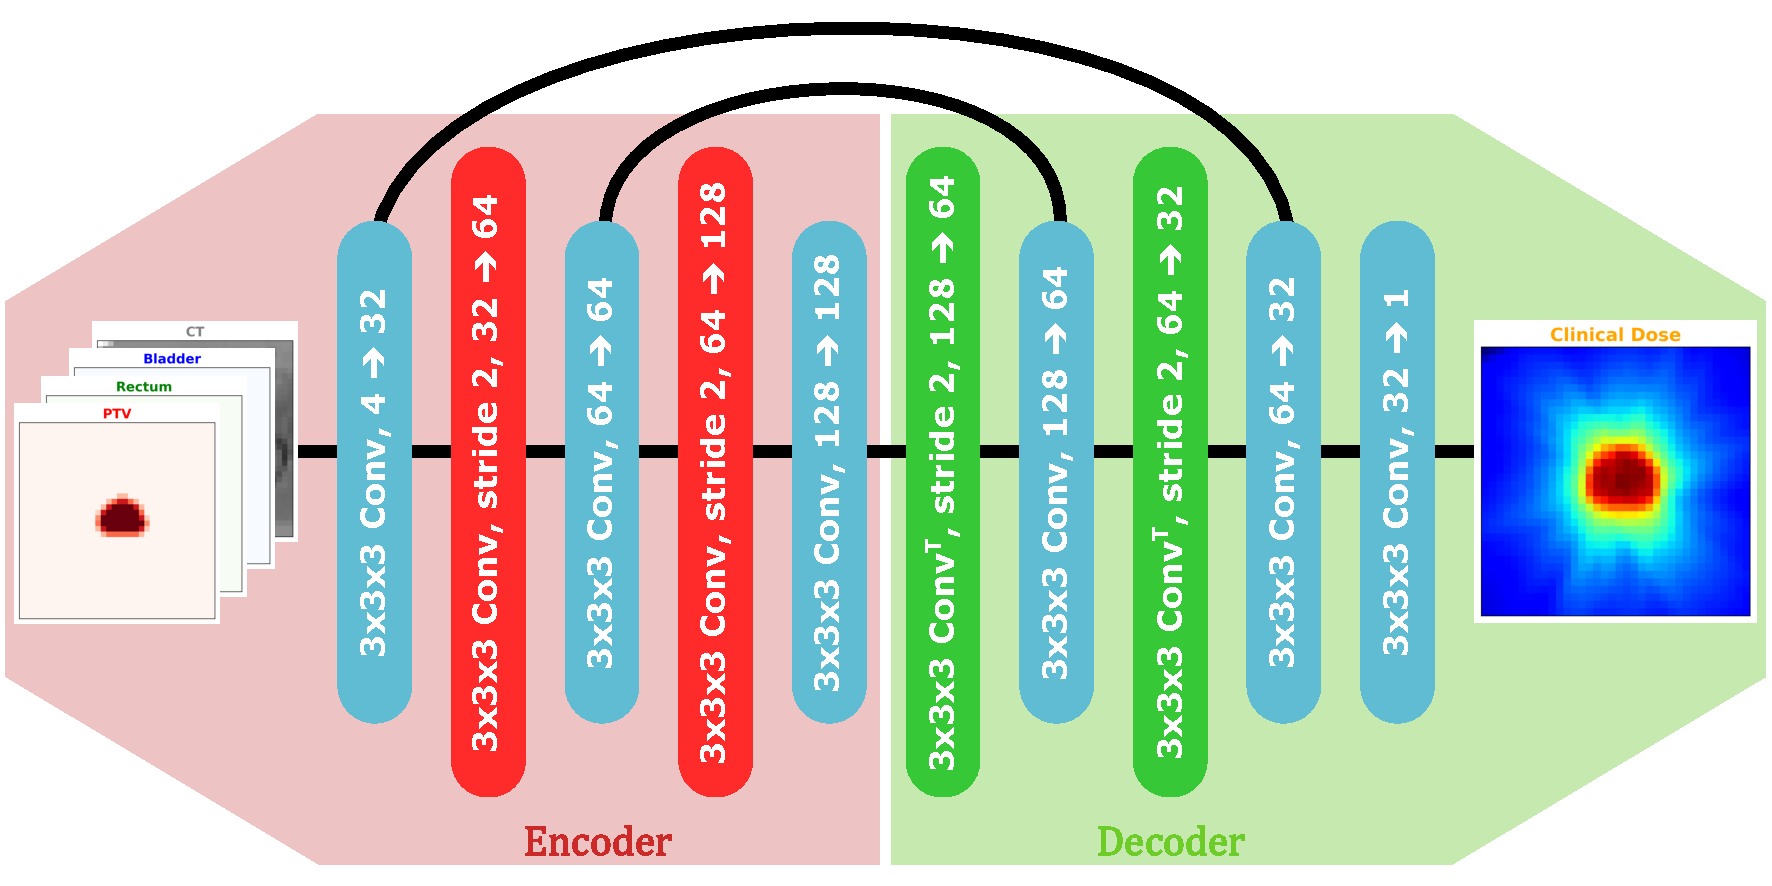
\includegraphics[width=11.5cm]{SFPM/modelC.pdf}
		\caption{Model C: No DVH data, \textbf{classical} U-net.}
		\label{fig:model_C_architecture}
	\end{subfigure}
	\begin{subfigure}{\linewidth}
		\centering
		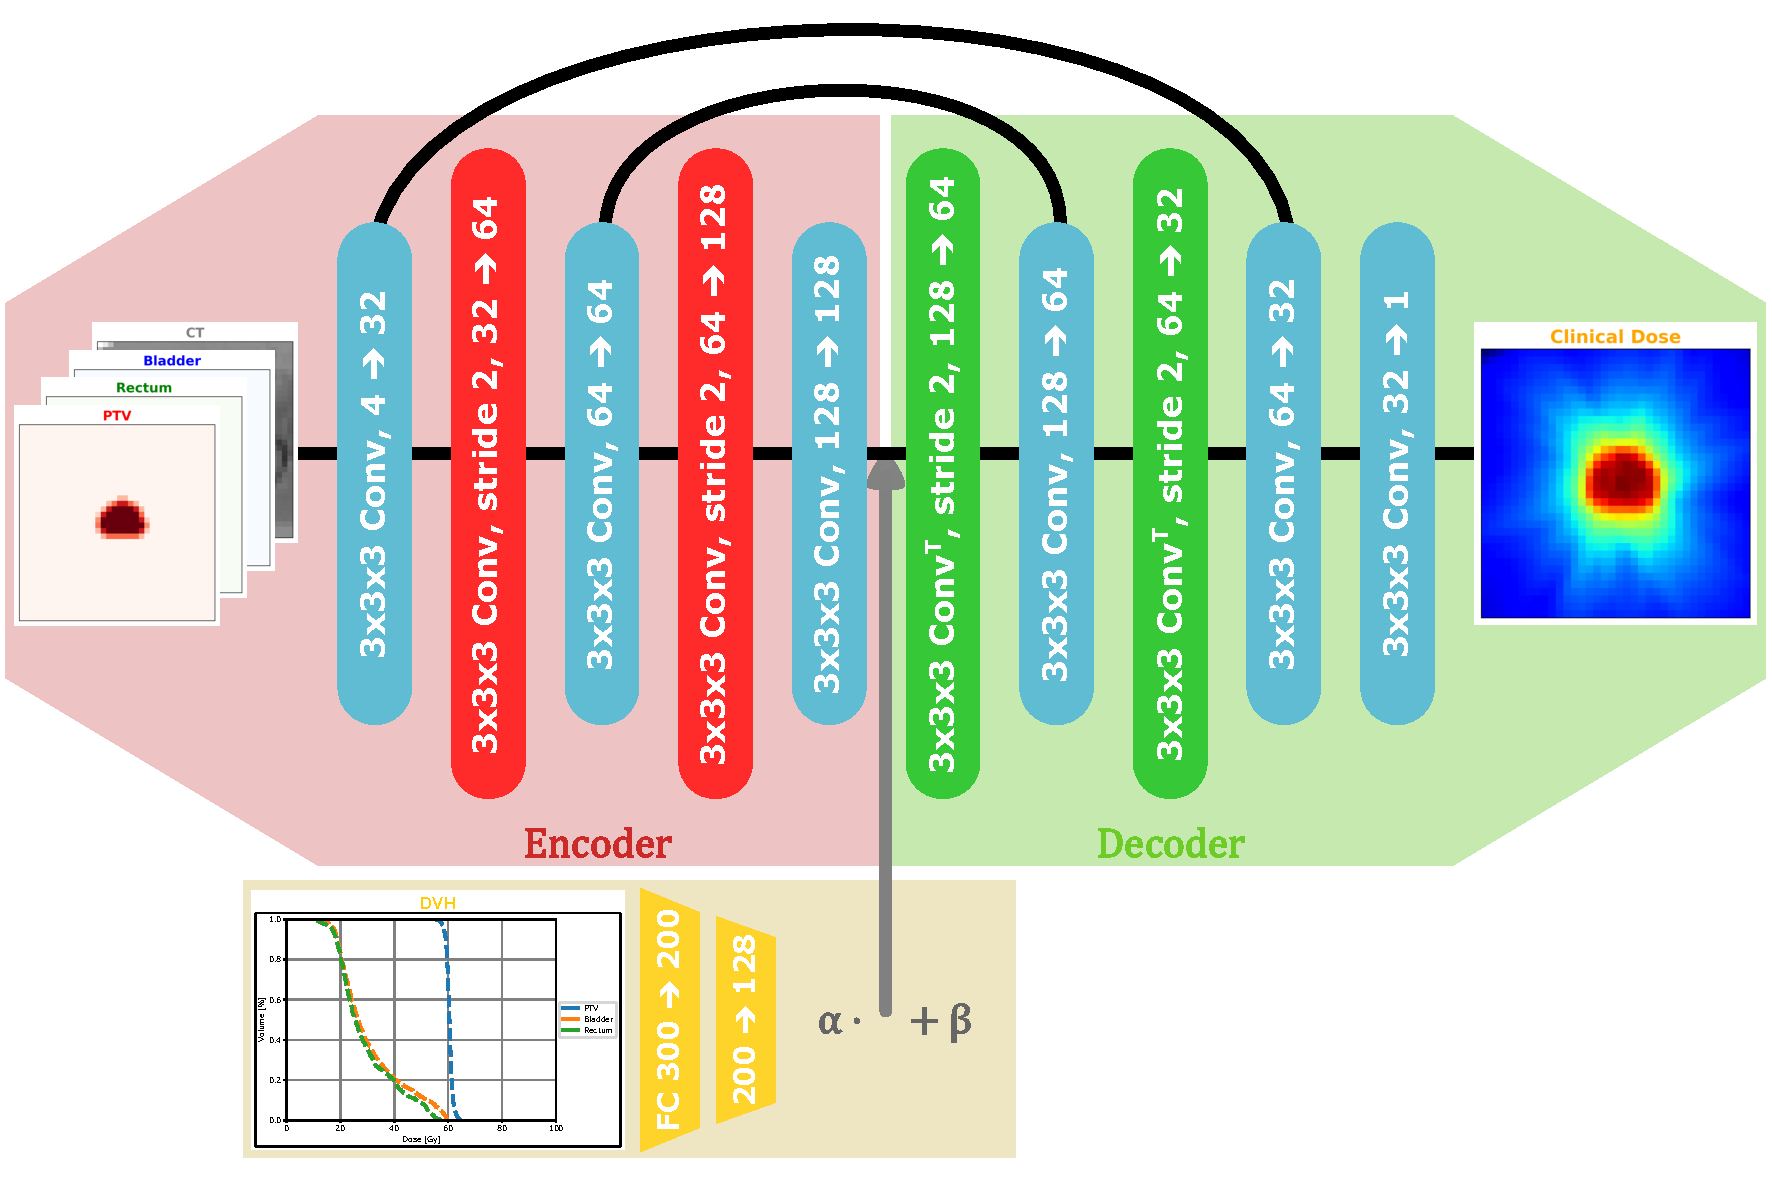
\includegraphics[width=11.5cm]{SFPM/modelB.pdf}
		\caption{Model B: DVH data using DAFT on the \textbf{bottleneck} of the U-net.}
		\label{fig:model_B_architecture}
	\end{subfigure}
	\begin{subfigure}{\linewidth}
		\centering
		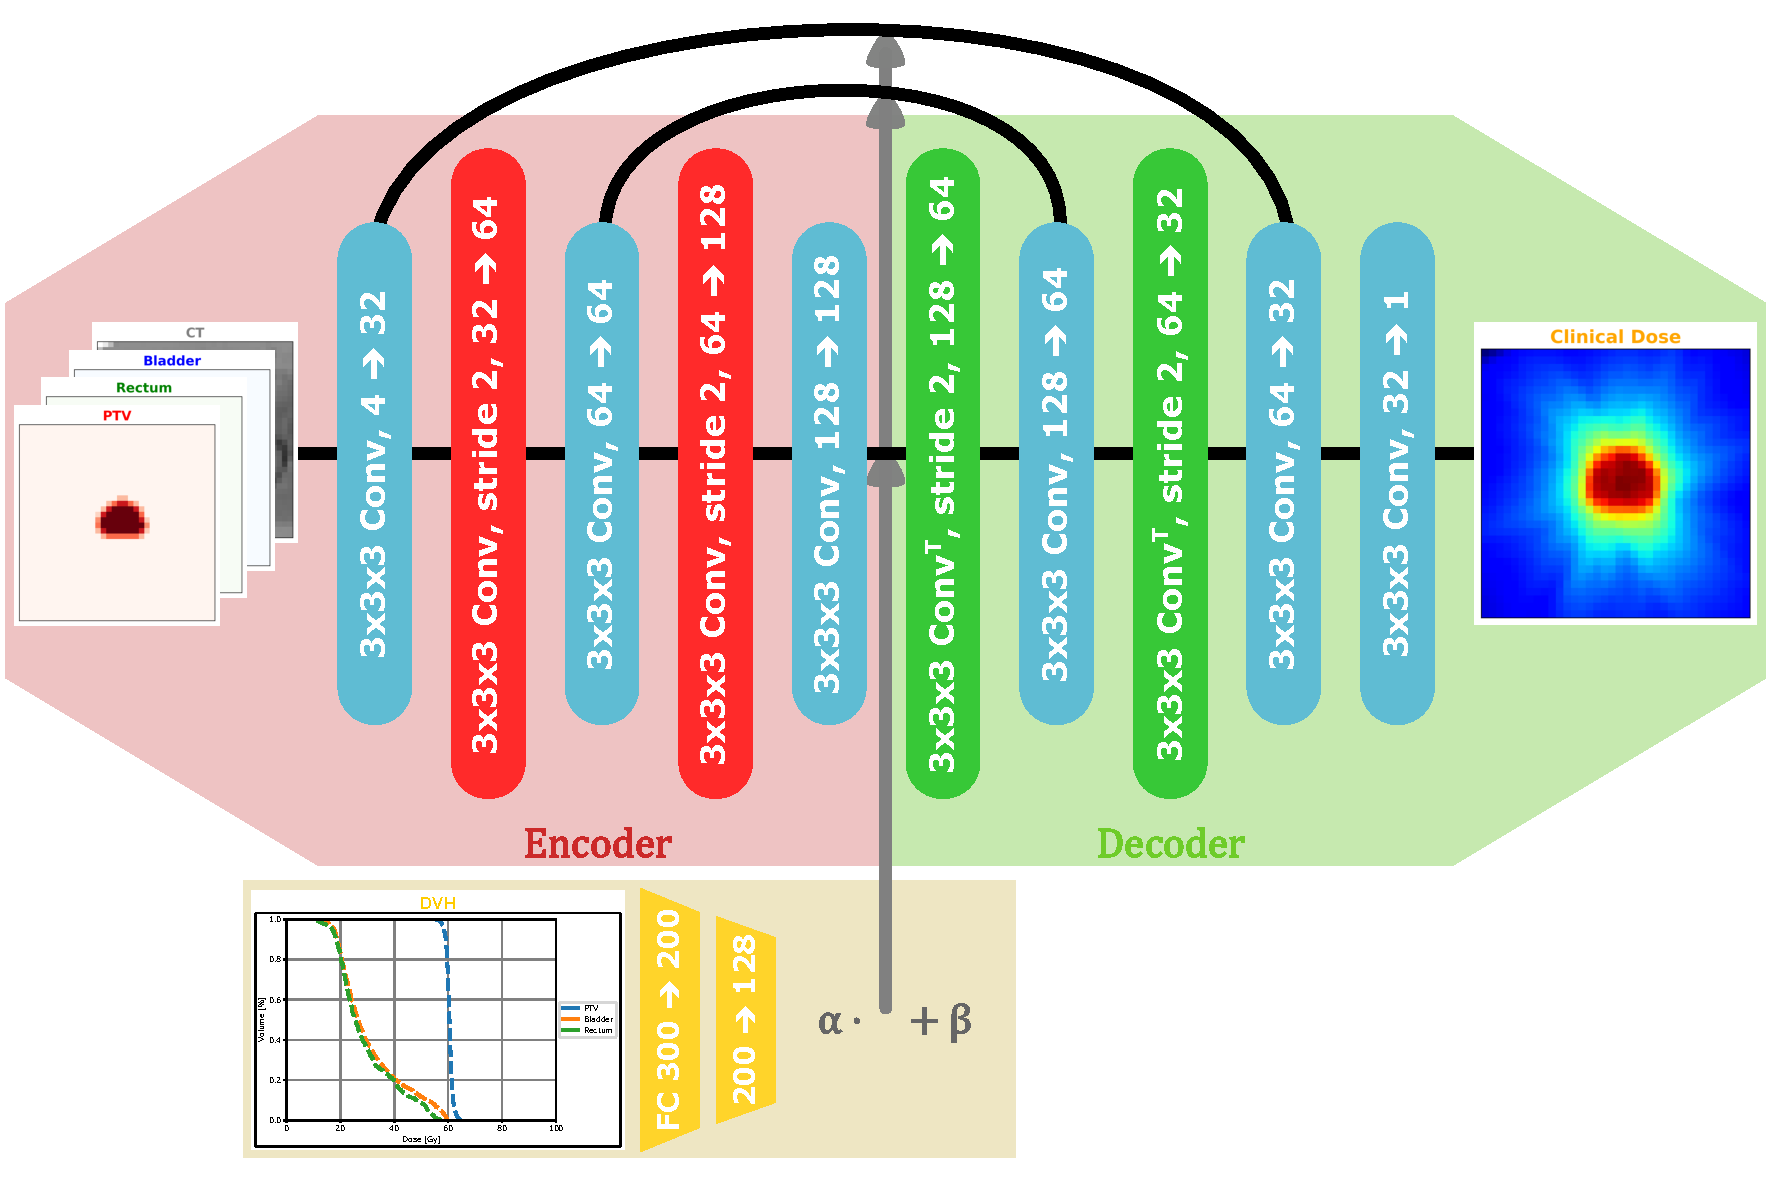
\includegraphics[width=11.5cm]{SFPM/modelA.pdf}
		\caption{Model A: DVH data using DAFT on all connections between the encoder and the decoder part of the U-net.}
		\label{fig:model_A_architecture}
	\end{subfigure}
	\caption{Architecture diagram of models A, B and C.}
	\label{fig:models_ABC_architectures}
\end{figure}

The first model referred to as "C" or the \textit{classic} model (figure \ref{fig:model_C_architecture}), consists of a standard 3D U-net architecture without any incorporation of DVH information.
The second model denoted as "B" or the \textit{bottleneck} model (figure \ref{fig:model_B_architecture}), integrates target DVH data using the DAFT technique, as described previously, at the bottleneck layer of the U-net.
In the third model, termed "A" or the \textit{all connections} model (figure \ref{fig:model_A_architecture}), DVH information is incorporated via the DAFT technique both at the bottleneck layer and across all skip connections between the encoder and decoder of the U-net.
During the model training process, the clinical DVHs corresponding to the real delivered doses were used as target DVHs for the optimization.

\subsection{Results}
Our results indicate that incorporating DVH data improves dose prediction's quantitative and qualitative aspects.

\paragraph{Quantitative Performance}
We used the Mean Absolute Error (MAE) between the predicted and ground-truth dose distributions to evaluate model performance.
The incorporation of dose-volume histogram data into the networks resulted in improved quantitative performance.
The MAE measured on the test dataset was $2.42\,\text{Gy}$ for model A, $2.58\,\text{Gy}$ for model B, and $3.18\,\text{Gy}$ for model C.

\paragraph{Prescription Adaptation}
\begin{figure}
	\centering
	\textit{(Solid line is predicted dose DVH, dotted line is target dose DVH.)}
	\begin{subfigure}{\linewidth}
		\centering
		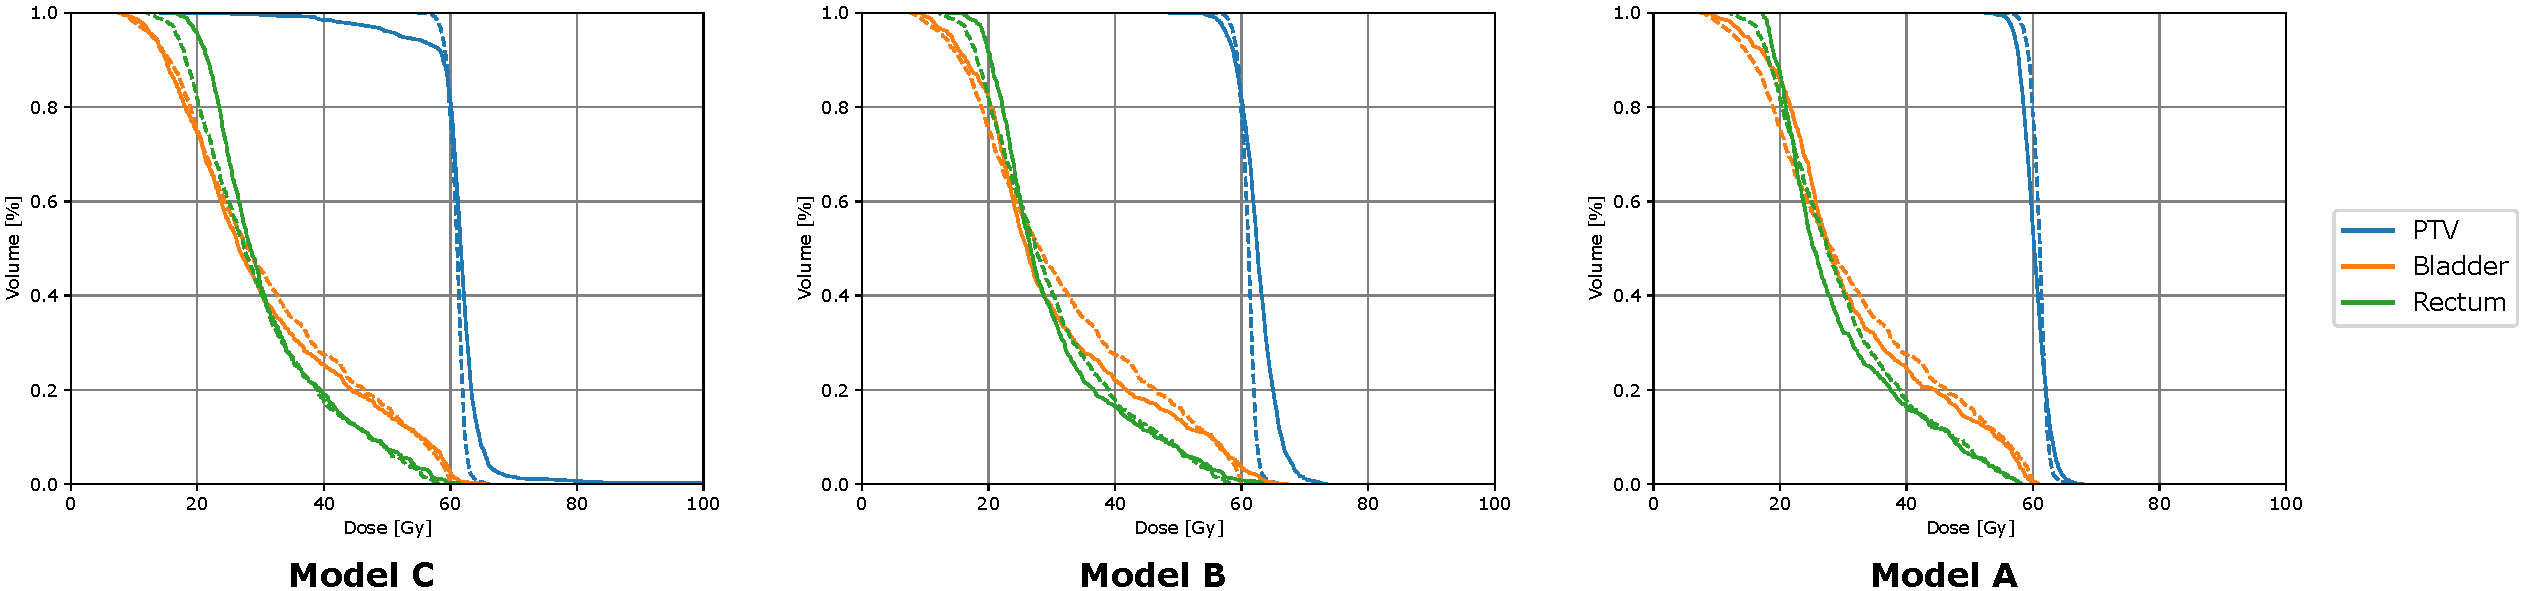
\includegraphics[width=\linewidth]{SFPM/test_patient_0.pdf}
		\caption{Patient 1, prescribed $62\,\text{Gy}$.}
		\label{fig:results_patient_1}
	\end{subfigure}
	\begin{subfigure}{\linewidth}
		\centering
		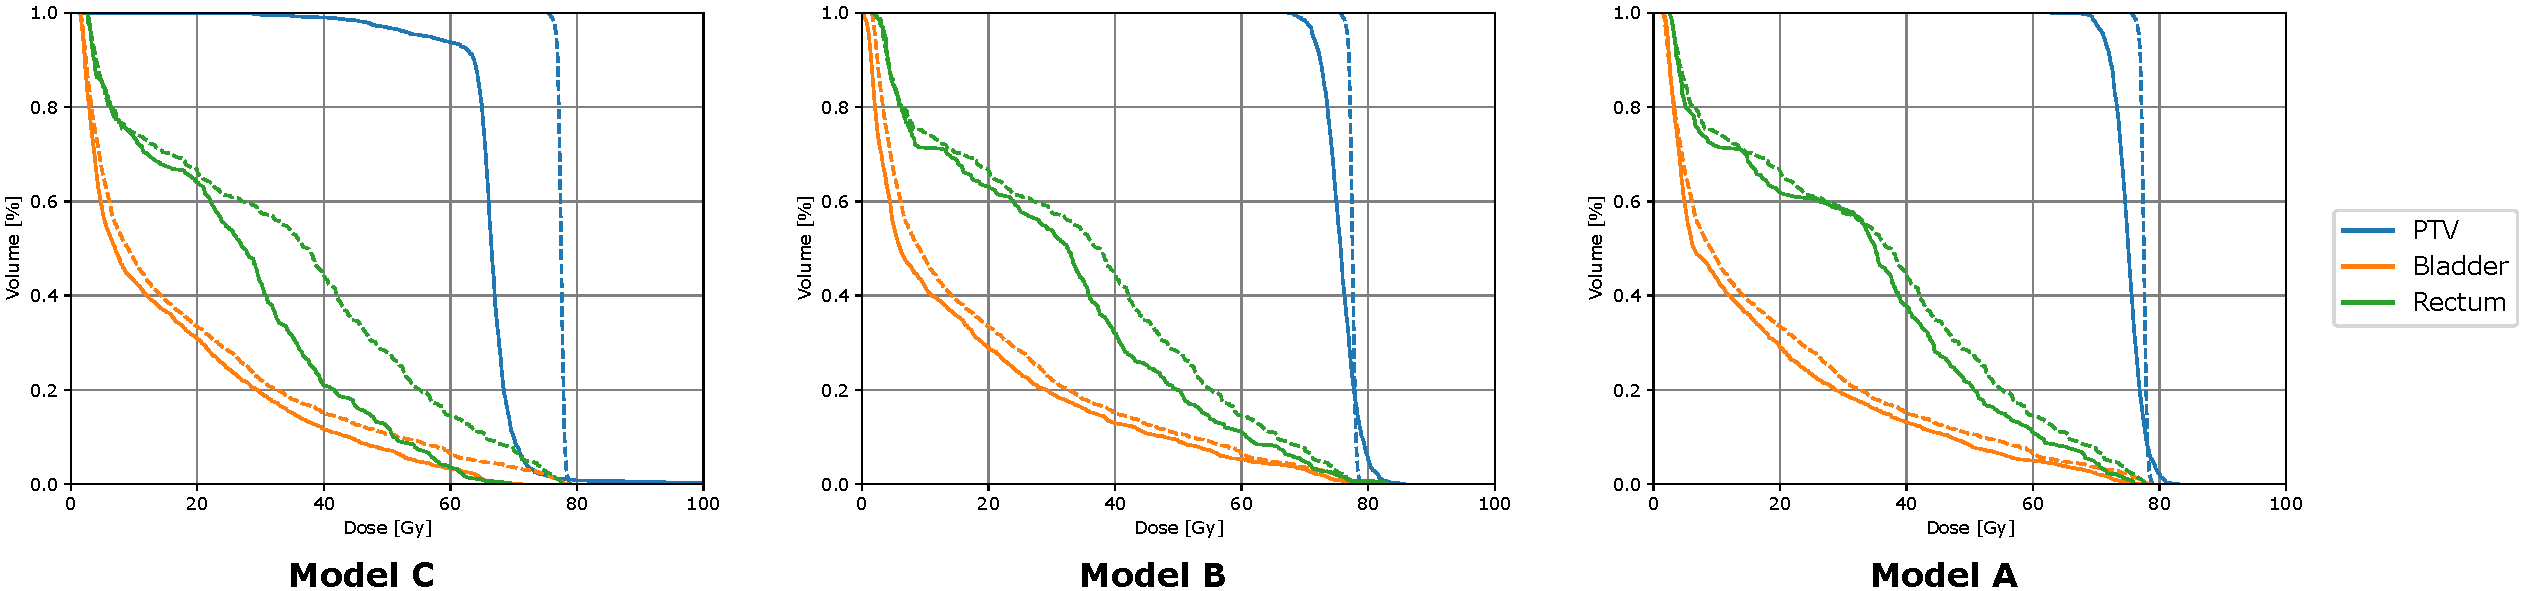
\includegraphics[width=\linewidth]{SFPM/test_patient_2.pdf}
		\caption{Patient 2, prescribed $78\,\text{Gy}$}
		\label{fig:results_patient_2}
	\end{subfigure}
	\caption{DVHs of the dose predicted by each model on two test set patients.}
	\label{fig:results_patients_12}
\end{figure}
In addition to the quantitative improvements, a qualitative analysis of the DVHs associated with the predicted dose distributions confirmed the benefit of including DVH information.
A key finding from our study was that models A and B could adapt their deep dose predictions based on the prescribed dose, with model A showing a slight advantage over model B regarding accuracy (see figure \ref{fig:results_patients_12}).
The dataset comprised patients with two distinct prescription doses: $62\,\text{Gy}$ and $78\,\text{Gy}$ to the PTV.
Model C consistently predicted dose distributions resembling a $65\,\text{Gy}$ prescription, demonstrating a lack of adaptability to the varying prescription levels (see figure \ref{fig:results_patients_12}).
In contrast, models A and B displayed greater flexibility, successfully adjusting their dose predictions following the prescribed doses for each patient.
This adaptive behavior highlights the effectiveness of incorporating DVH information, allowing the models to tailor dose predictions to specific prescription requirements.

\paragraph{Clinical Relevance}
The ability to adjust dose predictions based on DVH data demonstrates a significant advantage of our approach.
The prescription dose can vary in clinical practice depending on the tumor type, stage, and patient characteristics.
By incorporating DVH data, our models provide a more flexible and personalized approach to dose prediction, allowing the TPS to generate a plan that aligns with clinical objectives and dosimetrist input.

\subsection{Conclusions}
Our study shows the importance of incorporating DVH information into deep learning-based dose prediction models.
In this study, the target DVH links the clinical objectives defined by the dosimetrist and the predicted dose distribution.
We create a system allowing center-dependent adjustments by embedding this information into the model.
This system also allows interactive adjustment of the dose distribution when the proposed treatment plan is close to clinically acceptable.
The comparison of models A, B, and C highlights the advantages of integrating DVH data in the network.
The comparison also shows that integrating the information once at the bottleneck is sufficient.

An additional advantage of the proposed method is the capacity to generate standardized target DVH templates for treatment planning.
While averaging 3D dose distributions across multiple patients is not feasible, it is possible to compute average DVHs.
These average DVHs can be stratified by anatomical site, prescription dose, and clinical practice, providing a target for dose prediction with no effort.
Dosimetrists and doctors can further modify these templates to meet specific clinical requirements in case of non-standard patients.
Once an optimal set of DVHs is established for a given center's protocols, it can be reused for future patients with only minor adjustments.
Furthermore, sharing dose templates and treatment protocols from leading centers will allow knowledge transfer and elevate the quality of care in less-resourced hospitals.
This framework could enhance the efficiency and consistency of the treatment planning process.

Our proposed approach demonstrates the feasibility and benefits of incorporating DVH data into deep learning-based dose prediction models for radiotherapy treatment planning.
By embedding DVH information, we improve dose prediction accuracy and allow for interactive fine-tuning based on clinical objectives.
This technique opens the door to a new workflow where dosimetrists can design target DVHs, and the TPS generates the deliverable treatment plan that best matches these targets.
Further studies will explore the generalizability of our model across different cancer types and radiotherapy modalities.
Additionally, clinical validation studies will be crucial to assess the real-world impact of our proposed method on treatment outcomes and workflow efficiency.



%%%%%%%%%%%%%%%%%%%%%%%%%%%%%%%%%%%%%%%%%%%%%%%%%%%%%%%%%%%%%%%%%%%%%%%%
%                                                                      %
%   %%%%%%%%%%%%%%%%%%%%%%%%%%%%%%%%%%%%%%%%%%%%%%%%%%%%%%%%%%%%%%%%   %
%   %%%%%%%%%%%%%%%%%%%%%%%%%%%%%%%%%%%%%%%%%%%%%%%%%%%%%%%%%%%%%%%%   %
%   %%%%%%%%%%%%%%%%%%%%%%%%%%%%%%%%%%%%%%%%%%%%%%%%%%%%%%%%%%%%%%%%   %
%   %%%%%%%%%%%%%%%%%%%%%%%%%%%%%%%%%%%%%%%%%%%%%%%%%%%%%%%%%%%%%%%%   %
%                                                                      %
%%%%%%%%%%%%%%%%%%%%%%%%%%%%%%%%%%%%%%%%%%%%%%%%%%%%%%%%%%%%%%%%%%%%%%%%



% https://github.com/pauldubois98/SFRO2024
\section[Attention Mechanism on DVH for DeepDose]{Attention Mechanism on Dose-Volume Histograms for Deep Dose Predictions\footnote{Presented at SFRO 2024.}}
\subsection{Introduction}
This study builds on work from the previous section
We explore using attention mechanisms to improve the incorporation of target Dose-Volume Histogram information into deep-learning models for radiotherapy dose prediction.
In traditional radiotherapy planning, DVHs are essential for assessing and optimizing dose distributions for the Principal Target Volume and Organs at Risk.
However, existing deep learning models for dose prediction, while capable of generating accurate 3D dose distributions, often fail to integrate DVH constraints fully \cite{Pan2023}.
This limitation reduces their utility in real-time treatment planning.

In previous work, deep learning approaches primarily focused on predicting dose distributions directly from patient imaging data, such as CT scans and anatomical contours of the PTV and OARs.
These methods typically rely on convolutional neural networks (CNNs), like the Unet, trained with voxel-wise loss functions \cite{Ronneberger2015}.
While successful in producing accurate 3D dose maps, they generally treat DVH-related information as secondary, with little attention given to adapting predictions based on these critical clinical metrics.

In the last section, we proposed integrating target DVH into the deep dose model to address this gap.
In this section, we extend prior approaches by proposing attention mechanisms to integrate target DVH information more effectively into the dose prediction process.
Attention mechanisms, widely adopted in domains such as natural language processing and image recognition, enable models to focus on relevant features within the input data selectively \cite{Niu2021}.
By leveraging attention, we aim to enhance the model's capacity to dynamically adapt its dose predictions following specified DVH constraints, providing a more precise and clinically responsive framework for radiotherapy treatment planning.

This work evaluates three U-net-based architectures, including a novel model using a cross-attention mechanism to incorporate DVH information into the dose prediction process directly.
Our goal is to enhance the accuracy and adaptability of deep learning models for dose prediction, ultimately enabling dosimetrists to have greater control over the treatment planning process through DVH-guided model interactions.

\paragraph{Related work}
Previous studies have explored the application of attention mechanism for dose prediction in radiotherapy planning.
Osman et al., for example, developed an attention-gated 3D U-Net architecture model to predict full 3D dose distribution \cite{Osman2022}.
Cros et al. investigated the combination of dense elements with attention mechanisms for 3D radiotherapy dose prediction \cite{Ahmed2017}.
In contrast, our research uses the attention mechanism for its power in mixing different data types.
We used cross attention between DVH features and bottle neck compressed 3D data to predict clinically acceptable dose distributions.
To our knowledge, this innovative paradigm has not been previously explored in the literature.

\subsection{Material and Methods}
\paragraph{Patient Data and Preprocessing}
We again used the cohort of 168 patients from the previous section who had undergone radiotherapy treatment.
The dataset included patients prescribed 62 Gy or 78 Gy on the PTV.
The dataset was randomly split into 80\% for training, 10\% for validation, and 10\% for testing.
We collected the CT scans, PTV contours, and OAR contours for each patient.
The CT data was resampled to a voxel size of $0.5 \times 0.5 \times 0.5 \textit{mm}^3$ to standardize inputs across patients.
As in the last section, we used the same box $120 \times 180 \times 180\ \text{mm}^3$ centered on the PTV.

\paragraph{Model Architecture and Training}
The backbone architecture for all models in this study is a 3D-convolutional Unet, a commonly used CNN for image-to-image translation tasks, such as segmentation and dose prediction.
Our U-net is of depth two, meaning it performs two levels of down-sampling and up-sampling.
The U-net outputs a 3D dose prediction for each voxel within the patient's anatomy.
Details architecture diagrams can be found in figure \ref{fig:unets012}.

\subparagraph{U-net 0 (Baseline)}
The first model, U-net 0 (architecture diagram can be found on figure \ref{fig:unet0}), serves as a baseline and does not incorporate target DVH information.
It receives the CT scan, PTV, and OAR contours as input and predicts the 3D dose distribution purely from this spatial data.

\subparagraph{U-net 1 (DVH with DAFT)}
The second model, U-net 1 (architecture diagram can be found on figure \ref{fig:unet1}), incorporates DVH data using the DAFT approach, like in the previous section.
In this model, the target DVHs are provided as additional inputs, and the model is trained to predict 3D dose distributions that match these target DVHs.

\subparagraph{U-net 2 (DVH with Cross-Attention)}
Our novel contribution, U-net 2 (architecture diagram can be found on figure \ref{fig:unet2}), integrates DVH data using a cross-attention mechanism.
In this architecture, the model takes queries from the 3D dose prediction and keys and values from the target DVHs.
The result of the 4-head attention mechanism is the same shape as that of the 3D input.
The cross-attention mechanism allows the model to adjust its dose predictions dynamically based on the desired DVH information.
The output of the attention mechanism is re-injected into the U-net during the decoding process, modifying the predicted dose map to match the target DVHs better.

\begin{figure}
	\centering
	\vspace{-0.5cm}
	\begin{subfigure}{\linewidth}
		\centering
		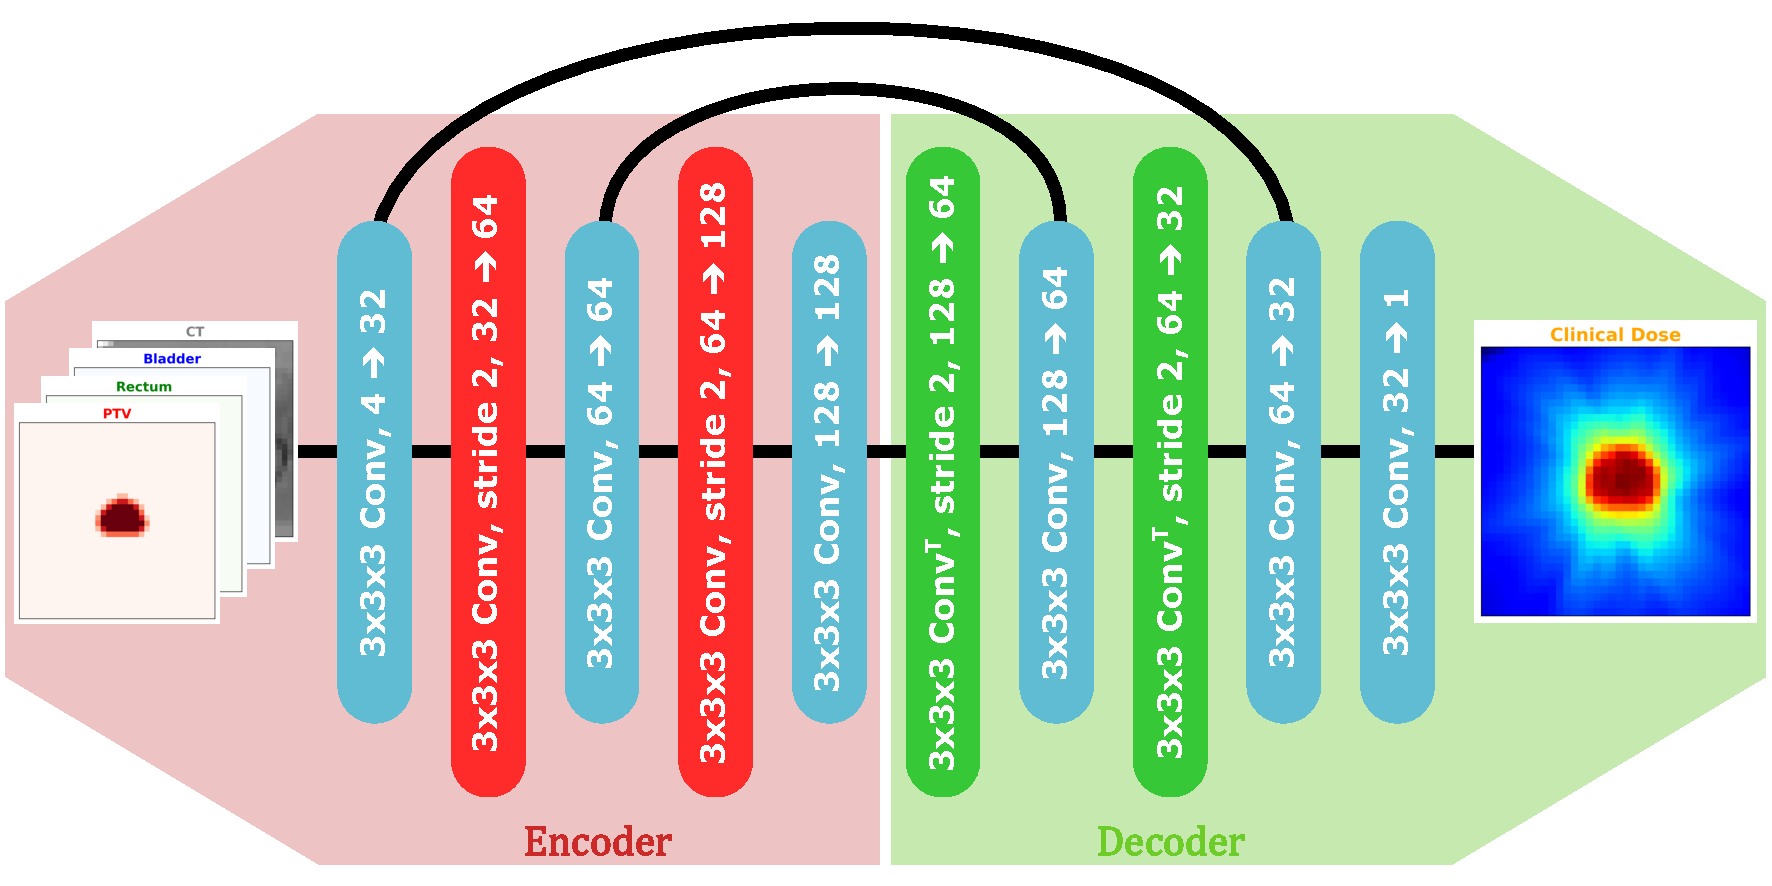
\includegraphics[width=12cm]{SFRO/model0.pdf}
		\caption{U-net 0: no DVH information.}
		\label{fig:unet0}
	\end{subfigure}
	\vspace{0.5cm}
	
	\begin{subfigure}{\linewidth}
		\centering
		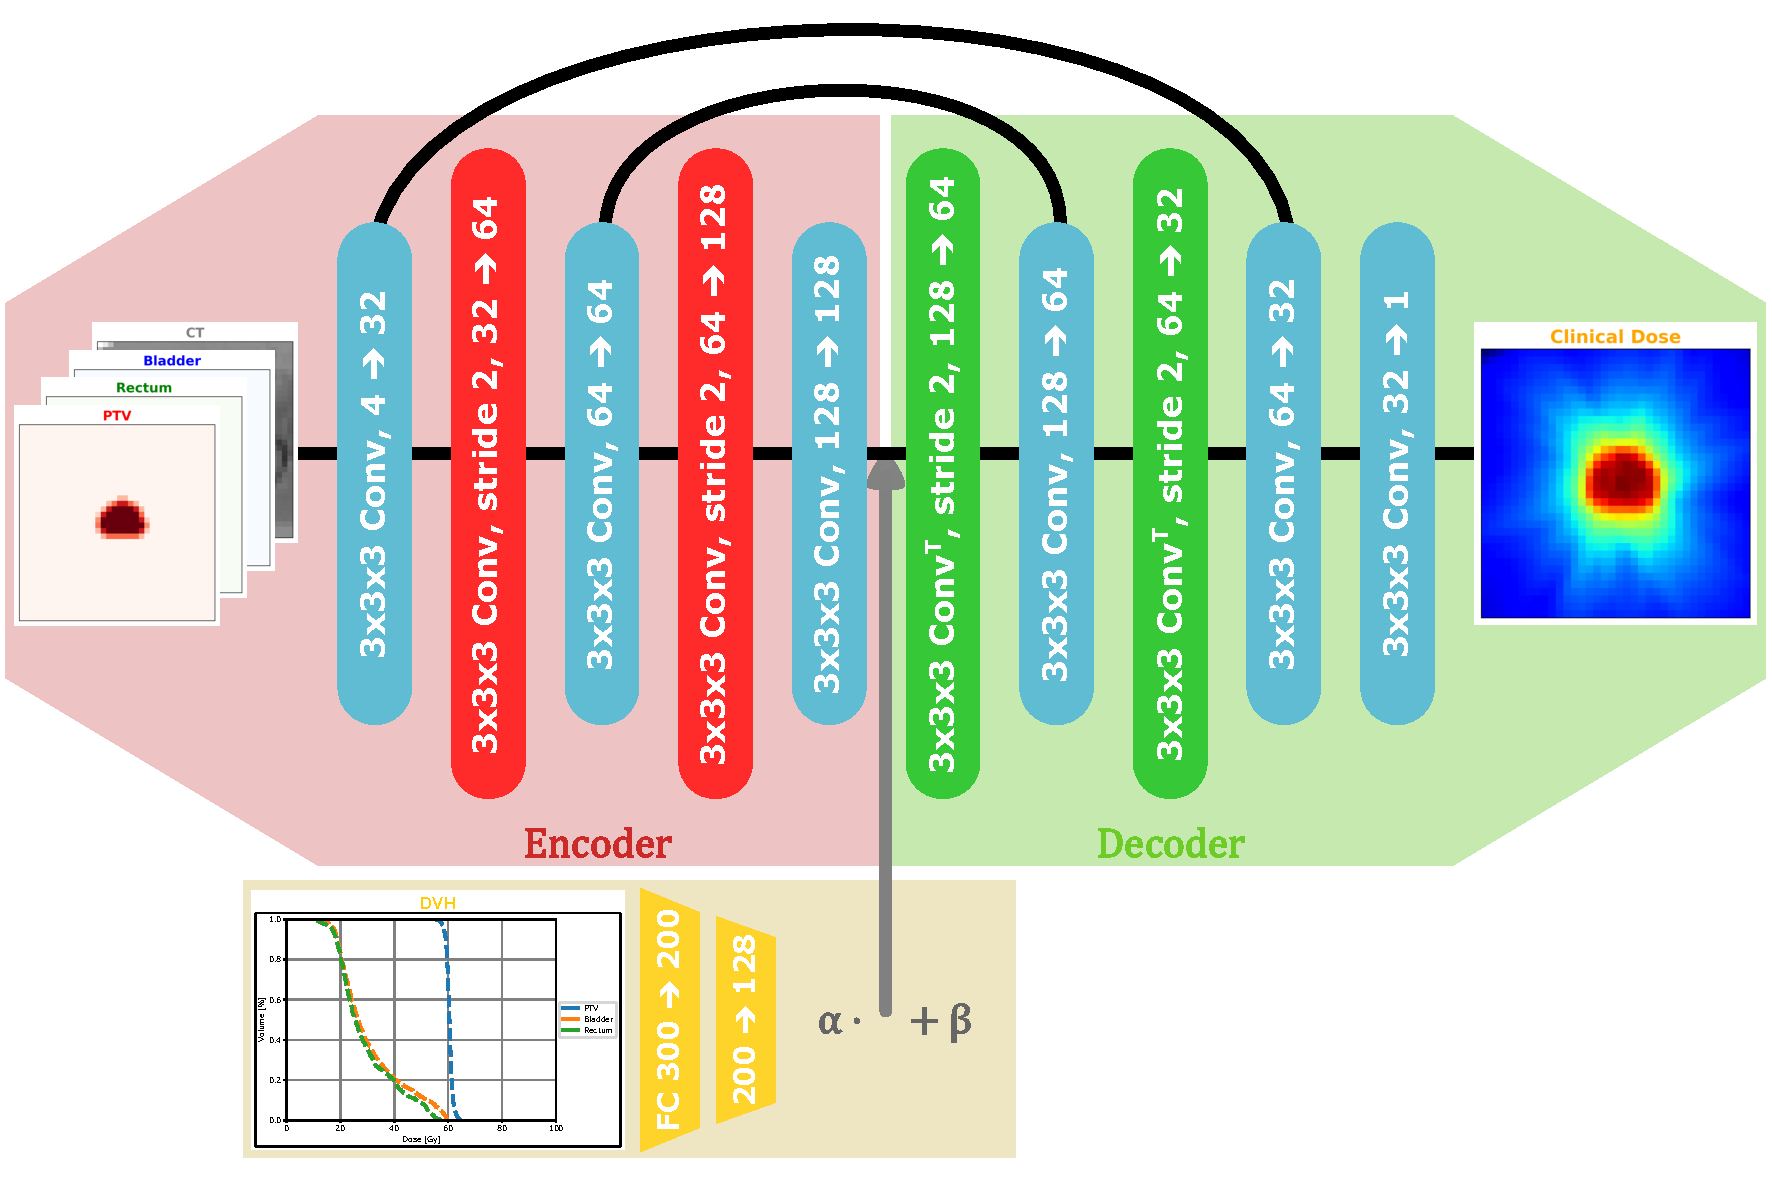
\includegraphics[width=12cm]{SFRO/model1.pdf}
		\caption{U-net 1: DVH with DAFT.}
		\label{fig:unet1}
	\end{subfigure}
	\vspace{0.5cm}
	
	\begin{subfigure}{\linewidth}
		\centering
		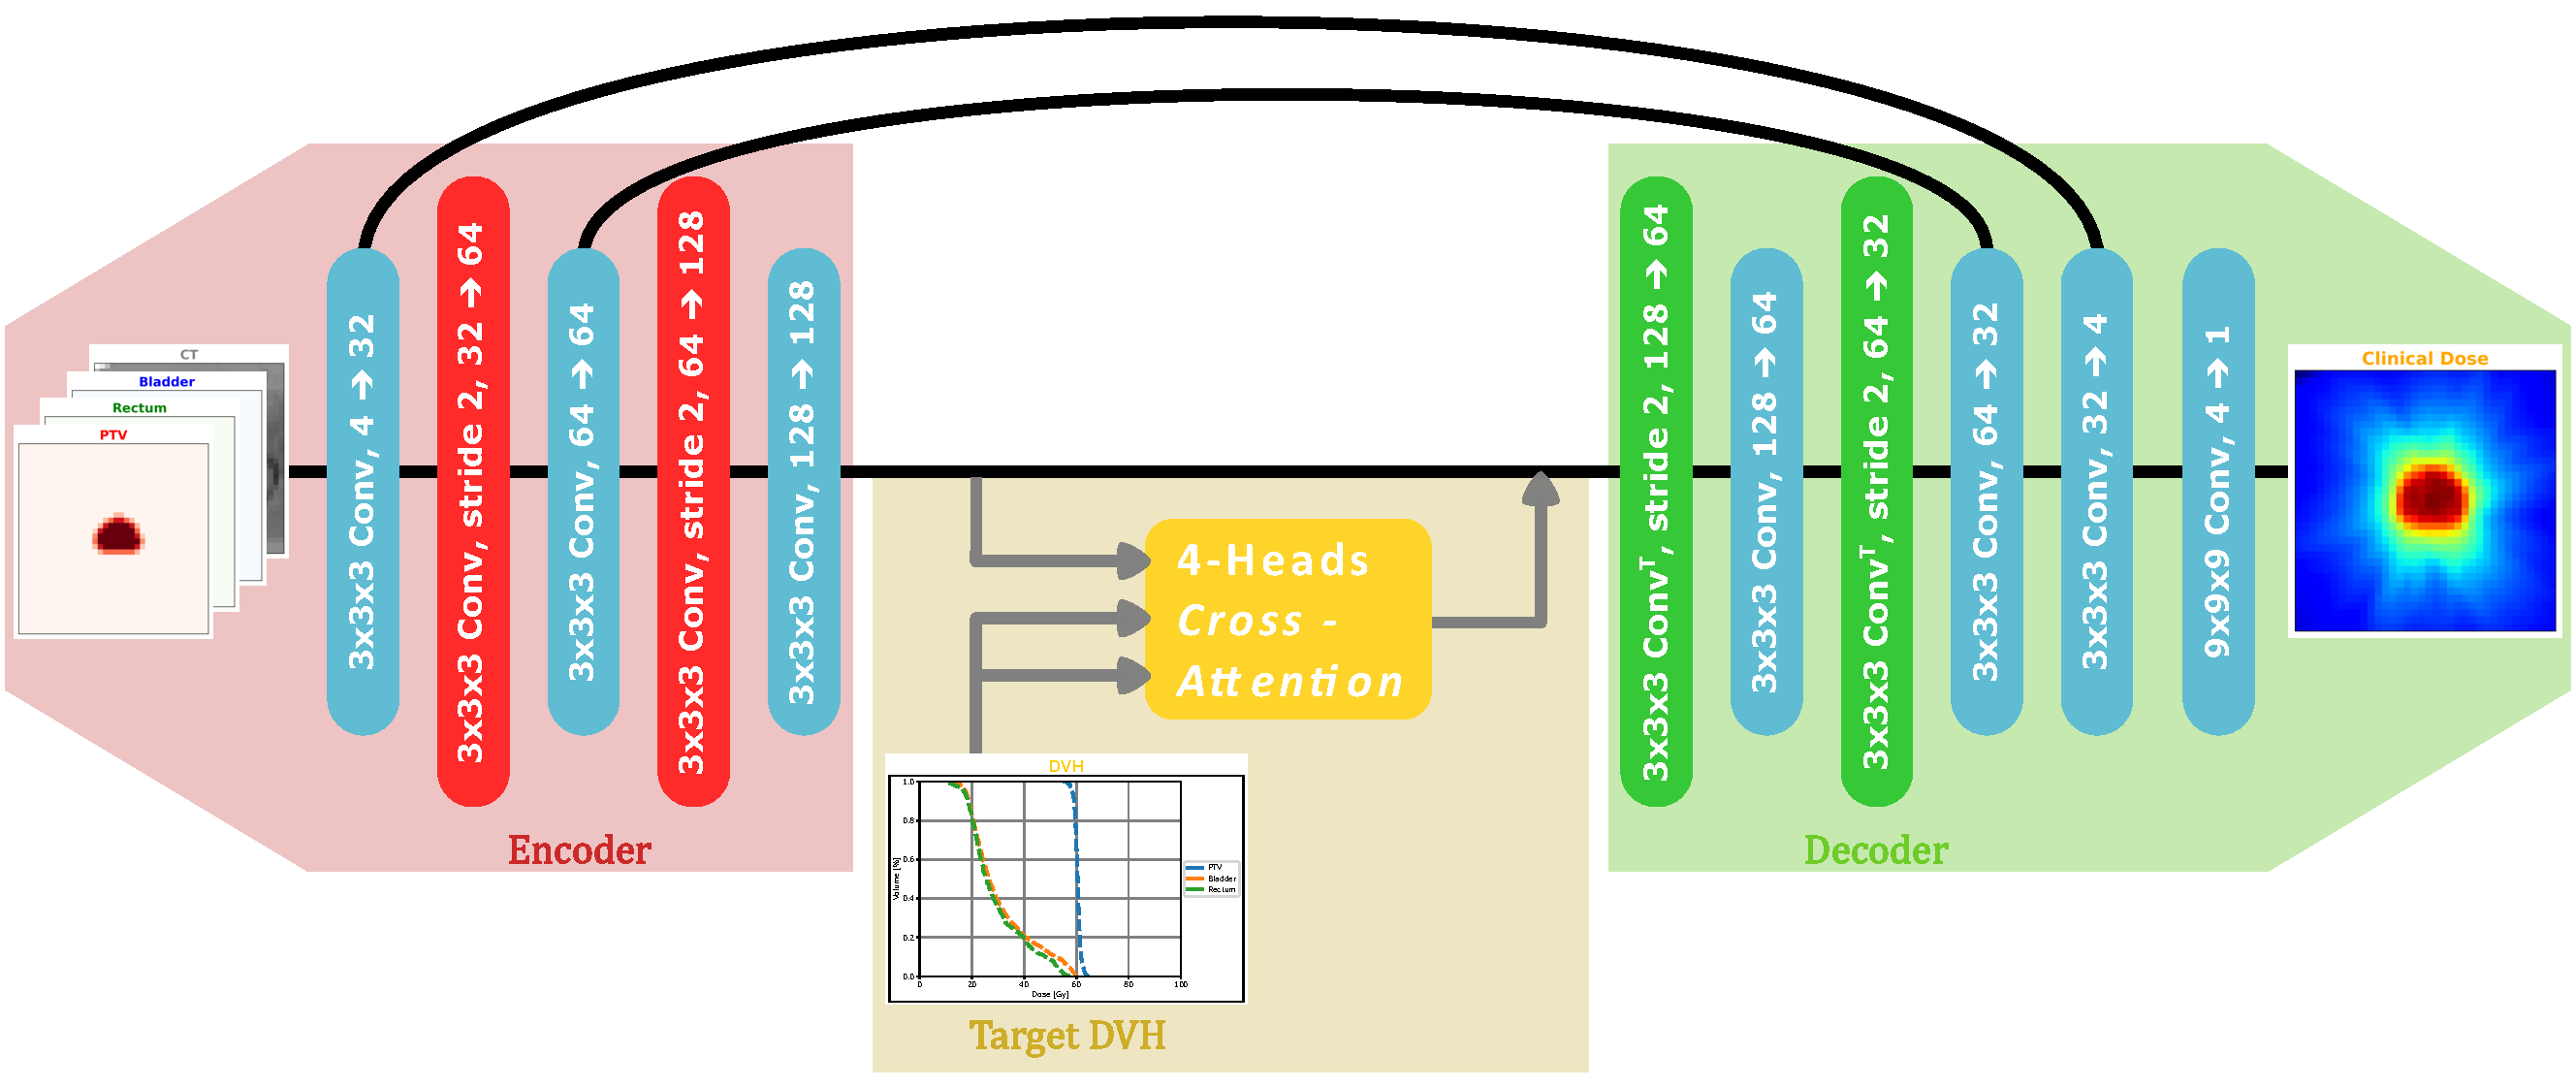
\includegraphics[width=12cm]{SFRO/model2.pdf}
		\caption{U-net 2: DVHs with cross-attention.}
		\label{fig:unet2}
	\end{subfigure}
	\caption{Architecture diagrams of U-nets 0, 1 and 2.}
	\label{fig:unets012}
\end{figure}

\paragraph{Loss Function and Optimization}
The models were trained using a loss function that combines voxel-wise MAE with an L1 loss on the DVH, designed to penalize deviations between the predicted and target DVHs.
Incorporating the L1 loss on DVH significantly improved the model’s convergence.
The total loss function is expressed as:
$$
\text{Total Loss} = \alpha \cdot \text{MAE}_{\text{voxel}} + \beta \cdot \text{L1}_{\text{DVH}}
$$
where $\alpha$ and $\beta$ are hyper-parameters that control the relative contribution of the two terms.
For this study, we set both $\alpha$ and $\beta$ to $1$, based on performance observed on the validation set.
However, future work could further optimize these parameters to enhance model performance.

The models were trained using the Adam optimizer with a $10^{-4}$ learning rate.
Using the validation loss criterion, early stopping was applied to prevent overfitting and ensure robust generalization.

\subsection{Results}
\paragraph{Evaluation Metrics}  
The performance of the models was assessed using two primary metrics.
The first metric was the 3D Dose MAE, which measures the voxel-wise MAE between the predicted dose distributions and the corresponding ground truth values.
The second metric was the DVH deviation, calculated as the mean L1 deviation between the predicted and target DVHs for both the Principal Target Volume (PTV) and Organs at Risk (OARs).
These metrics provide a comprehensive evaluation of the models' accuracy in predicting dose distributions and adherence to clinical DVH constraints.

\paragraph{Models Performances}
The performance of the three models is summarized in Table \ref{tab:model_performance}.
Both U-net 1 and U-net 2, which incorporated DVH information, outperformed the baseline U-net 0 across all metrics.

\begin{table}
	\centering
	\begin{tabular}{|l|c|c|c|}
		\hline
		\textbf{Metric}         & \textbf{Unet-0} & \textbf{Unet-1} & \textbf{Unet-2} \\
		\hline
		3D Dose MAE (Gy)        & 3.093           & 2.254           & 2.210           \\
		\hline
		Mean DVH Deviation (Gy) & 1.942           & 1.051           & 0.930           \\
		\hline
	\end{tabular}
	\caption{Models performances comparison.}
	\label{tab:model_performance}
\end{table}

As shown, the inclusion of DVH data significantly reduced the MAE in the predicted dose distributions.
Unet-2, which used a cross-attention mechanism, showed the best overall performance, with a minor error reduction compared to U-net 1.

\paragraph{Prescription Adaptability}
The ability of the models to adapt to varying prescriptions was also evaluated.
Similarly to the last section, U-net 0 struggled to predict the correct dose when the prescription varied from its training distribution.
Regardless of the actual prescription, the model consistently predicted doses around $65\,\textit{Gy}$.
In contrast, U-net 1 and U-net 2 adapted their dose predictions to the provided DVHs, making them more versatile in clinical scenarios where the prescription may differ across patients.
There were only a few differences between the performances of U-net 1 and U-net 2.

\subsection{Conclusions}
This study re-demonstrates the feasibility of incorporating DVH data into deep-learning models for radiotherapy dose prediction.
We have marginally improved model performances and adaptability by using an attention mechanism to integrate target DVHs.
The cross-attention mechanism, in particular, offers a novel way to align predicted dose distributions with clinical goals flexibly.

Our findings indicate that this approach could facilitate the development of a more efficient radiotherapy treatment planning workflow.
In this proposed framework, dosimetrists would focus primarily on creating standardized target DVH templates rather than manually adjusting dose distributions for each patient.
These templates would serve as a foundation, requiring minimal adjustments to accommodate individual patient-specific characteristics, thereby streamlining the treatment planning process.

Designing a template for 3D dose distributions is not feasible, as 3D doses are highly patient-specific and cannot be transferred between patients.
In contrast, DVHs are more generalizable and can be applied across different patients.
This generalizability makes them suitable for the proposed workflow, where template DVHs can be established and used with deep learning-based dose prediction models guided by target DVH.
This workflow could reduce planning time and improve consistency across patients.
Future work will explore incorporating more complex DVH structures and refining the attention mechanism to enhance model interpretability and clinical usability.
